\documentclass[journal,12pt,twocolumn]{IEEEtran}
\usepackage{setspace}
\usepackage{gensymb}
\usepackage{caption}
%\usepackage{multirow}
%\usepackage{multicolumn}
%\usepackage{subcaption}
%\doublespacing
\singlespacing
\usepackage{csvsimple}
\usepackage{amsmath}
\usepackage{multicol}
%\usepackage{enumerate}
\usepackage{amssymb}
%\usepackage{graphicx}
\usepackage{newfloat}
%\usepackage{syntax}
\usepackage{listings}
\usepackage{color}
\usepackage{tikz}
\usetikzlibrary{shapes,arrows}



%\usepackage{graphicx}
%\usepackage{amssymb}
%\usepackage{relsize}
%\usepackage[cmex10]{amsmath}
%\usepackage{mathtools}
%\usepackage{amsthm}
%\interdisplaylinepenalty=2500
%\savesymbol{iint}
%\usepackage{txfonts}
%\restoresymbol{TXF}{iint}
%\usepackage{wasysym}
\usepackage{amsthm}
\usepackage{mathrsfs}
\usepackage{txfonts}
\usepackage{stfloats}
\usepackage{cite}
\usepackage{cases}
\usepackage{mathtools}
\usepackage{caption}
\usepackage{enumerate}	
\usepackage{enumitem}
\usepackage{amsmath}
%\usepackage{xtab}
\usepackage{longtable}
\usepackage{multirow}
%\usepackage{algorithm}
%\usepackage{algpseudocode}
\usepackage{enumitem}
\usepackage{mathtools}
\usepackage{hyperref}
%\usepackage[framemethod=tikz]{mdframed}
\usepackage{listings}
    %\usepackage[latin1]{inputenc}                                 %%
    \usepackage{color}                                            %%
    \usepackage{array}                                            %%
    \usepackage{longtable}                                        %%
    \usepackage{calc}                                             %%
    \usepackage{multirow}                                         %%
    \usepackage{hhline}                                           %%
    \usepackage{ifthen}                                           %%
  %optionally (for landscape tables embedded in another document): %%
    \usepackage{lscape}     


\usepackage{url}
\def\UrlBreaks{\do\/\do-}


%\usepackage{stmaryrd}


%\usepackage{wasysym}
%\newcounter{MYtempeqncnt}
\DeclareMathOperator*{\Res}{Res}
%\renewcommand{\baselinestretch}{2}
\renewcommand\thesection{\arabic{section}}
\renewcommand\thesubsection{\thesection.\arabic{subsection}}
\renewcommand\thesubsubsection{\thesubsection.\arabic{subsubsection}}

\renewcommand\thesectiondis{\arabic{section}}
\renewcommand\thesubsectiondis{\thesectiondis.\arabic{subsection}}
\renewcommand\thesubsubsectiondis{\thesubsectiondis.\arabic{subsubsection}}

% correct bad hyphenation here
\hyphenation{op-tical net-works semi-conduc-tor}

%\lstset{
%language=C,
%frame=single, 
%breaklines=true
%}

%\lstset{
	%%basicstyle=\small\ttfamily\bfseries,
	%%numberstyle=\small\ttfamily,
	%language=Octave,
	%backgroundcolor=\color{white},
	%%frame=single,
	%%keywordstyle=\bfseries,
	%%breaklines=true,
	%%showstringspaces=false,
	%%xleftmargin=-10mm,
	%%aboveskip=-1mm,
	%%belowskip=0mm
%}

%\surroundwithmdframed[width=\columnwidth]{lstlisting}
\def\inputGnumericTable{}                                 %%
\lstset{
%language=C,
frame=single, 
breaklines=true,
columns=fullflexible
}
 

\begin{document}
%
\tikzstyle{block} = [rectangle, draw,
    text width=3em, text centered, minimum height=3em]
\tikzstyle{sum} = [draw, circle, node distance=3cm]
\tikzstyle{input} = [coordinate]
\tikzstyle{output} = [coordinate]
\tikzstyle{pinstyle} = [pin edge={to-,thin,black}]
\providecommand{\e}[1]{\ensuremath{E\left(#1\right)}}
\providecommand{\es}[1]{\ensuremath{E\left[#1\right]}}
\theoremstyle{definition}
\newtheorem{theorem}{Theorem}[section]
\newtheorem{problem}{Problem}
\newtheorem{proposition}{Proposition}[section]
\newtheorem{lemma}{Lemma}[section]
\newtheorem{corollary}[theorem]{Corollary}
\newtheorem{example}{Example}[section]
\newtheorem{definition}{Definition}[section]
%\newtheorem{algorithm}{Algorithm}[section]
%\newtheorem{cor}{Corollary}
\newcommand{\BEQA}{\begin{eqnarray}}
\newcommand{\EEQA}{\end{eqnarray}}
\newcommand{\define}{\stackrel{\triangle}{=}}
\bibliographystyle{IEEEtran}
%\bibliographystyle{ieeetr}
\providecommand{\nCr}[2]{\,^{#1}C_{#2}} % nCr
\providecommand{\nPr}[2]{\,^{#1}P_{#2}} % nPr
\providecommand{\mbf}{\mathbf}
\providecommand{\pr}[1]{\ensuremath{\Pr\left(#1\right)}}
\providecommand{\qfunc}[1]{\ensuremath{Q\left(#1\right)}}
\providecommand{\sbrak}[1]{\ensuremath{{}\left[#1\right]}}
\providecommand{\lsbrak}[1]{\ensuremath{{}\left[#1\right.}}
\providecommand{\rsbrak}[1]{\ensuremath{{}\left.#1\right]}}
\providecommand{\brak}[1]{\ensuremath{\left(#1\right)}}
\providecommand{\lbrak}[1]{\ensuremath{\left(#1\right.}}
\providecommand{\rbrak}[1]{\ensuremath{\left.#1\right)}}
\providecommand{\cbrak}[1]{\ensuremath{\left\{#1\right\}}}
\providecommand{\lcbrak}[1]{\ensuremath{\left\{#1\right.}}
\providecommand{\rcbrak}[1]{\ensuremath{\left.#1\right\}}}
\theoremstyle{remark}
\newtheorem{rem}{Remark}
\newcommand{\sgn}{\mathop{\mathrm{sgn}}}
\providecommand{\fourier}{\overset{\mathcal{F}}{ \rightleftharpoons}}
%\providecommand{\hilbert}{\overset{\mathcal{H}}{ \rightleftharpoons}}
\providecommand{\system}{\overset{\mathcal{H}}{ \longleftrightarrow}}
	%\newcommand{\solution}[2]{\textbf{Solution:}{#1}}
\newcommand{\solution}{\noindent \textbf{Solution: }}
\newcommand{\myvec}[1]{\ensuremath{\begin{pmatrix}#1\end{pmatrix}}}
\providecommand{\dec}[2]{\ensuremath{\overset{#1}{\underset{#2}{\gtrless}}}}
\DeclarePairedDelimiter{\ceil}{\lceil}{\rceil}
%\numberwithin{equation}{section}
%\numberwithin{problem}{subsection}
%\numberwithin{definition}{subsection}
\makeatletter
%\@addtoreset{figure}{section}
\makeatother
\let\StandardTheFigure\thefigure
%\renewcommand{\thefigure}{\theproblem.\arabic{figure}}
\renewcommand{\thefigure}{\thesection}
%\numberwithin{figure}{subsection}
%\numberwithin{equation}{subsection}
%\numberwithin{equation}{section}
%\numberwithin{equation}{problem}
%\numberwithin{problem}{subsection}
\numberwithin{problem}{section}
%%\numberwithin{definition}{subsection}
%\makeatletter
%\@addtoreset{figure}{problem}
%\makeatother
\makeatletter
%\@addtoreset{table}{section}
\makeatother
\let\StandardTheFigure\thefigure
\let\StandardTheTable\thetable
\let\vec\mathbf
\numberwithin{equation}{section}
\vspace{3cm}
\title{%Convex Optimization in Python
	{
	Random Numbers
	}
}
%\title{
%	\logo{Matrix Analysis through Octave}{\begin{center}\includegraphics[scale=.24]{tlc}\end{center}}{}{HAMDSP}
%}
% paper title
% can use linebreaks \\ within to get better formatting as desired
%\title{Matrix Analysis through Octave}
%
%
% author names and IEEE memberships
% note positions of commas and nonbreaking spaces ( ~ ) LaTeX will not break
% a structure at a ~ so this keeps an author's name from being broken across
% two lines.
% use \thanks{} to gain access to the first footnote area
% a separate \thanks must be used for each paragraph as LaTeX2e's \thanks
% was not built to handle multiple paragraphs
%
\author{ Aakash Kamuju}
% note the % following the last \IEEEmembership and also \thanks - 
% these prevent an unwanted space from occurring between the last author name
% and the end of the author line. i.e., if you had this:
% 
% \author{....lastname \thanks{...} \thanks{...} }
%                     ^------------^------------^----Do not want these spaces!
%
% a space would be appended to the last name and could cause every name on that
% line to be shifted left slightly. This is one of those "LaTeX things". For
% instance, "\textbf{A} \textbf{B}" will typeset as "A B" not "AB". To get
% "AB" then you have to do: "\textbf{A}\textbf{B}"
% \thanks is no different in this regard, so shield the last } of each \thanks
% that ends a line with a % and do not let a space in before the next \thanks.
% Spaces after \IEEEmembership other than the last one are OK (and needed) as
% you are supposed to have spaces between the names. For what it is worth,
% this is a minor point as most people would not even notice if the said evil
% space somehow managed to creep in.
% The paper headers
%\markboth{Journal of \LaTeX\ Class Files,~Vol.~6, No.~1, January~2007}%
%{Shell \MakeLowercase{\textit{et al.}}: Bare Demo of IEEEtran.cls for Journals}
% The only time the second header will appear is for the odd numbered pages
% after the title page when using the twoside option.
% 
% *** Note that you probably will NOT want to include the author's ***
% *** name in the headers of peer review papers.                   ***
% You can use \ifCLASSOPTIONpeerreview for conditional compilation here if
% you desire.
% If you want to put a publisher's ID mark on the page you can do it like
% this:
%\IEEEpubid{0000--0000/00\$00.00~\copyright~2007 IEEE}
% Remember, if you use this you must call \IEEEpubidadjcol in the second
% column for its text to clear the IEEEpubid mark.
% make the title area
\maketitle
\tableofcontents
\bigskip
\renewcommand{\thefigure}{\theenumi}
\renewcommand{\thetable}{\theenumi}
%template ends here
\section{Uniform Random Numbers}
Let $U$ be a uniform random variable between 0 and 1.
\begin{enumerate}[label=\thesection.\arabic*
,ref=\thesection.\theenumi]
\item Generate $10^6$ samples of $U$ using a C program and save into a file called uni.dat .
\\
\solution \\Download the following files and execute the  C program.
\begin{lstlisting}
wget https://github.com/kamujuaakash/Assignment1/blob/main/Exercise/Exercise-1/1.1/exrand.c
wget https://github.com/kamujuaakash/Assignment1/blob/main/Exercise/Exercise-1/1.1/coeffs.h
\end{lstlisting}
Download the above files and execute the following commands
\begin{lstlisting}
gcc exrand.c -lm
./a.out
\end{lstlisting}
\item
Load the uni.dat file into python and plot the empirical CDF of $U$ using the samples in uni.dat. The CDF is defined as
\begin{align}
F_{U}(x) = \pr{U \le x}
\end{align}
\\
\solution  \\The following code plots Fig. \ref{fig:1.2}
\begin{lstlisting}
wget https://github.com/kamujuaakash/Assignment1/blob/main/Exercise/Exercise-1/1.2/cdf_plot.py
\end{lstlisting}
Download the above files and execute the following commands to produce Fig.\ref{fig:1.2}
\begin{lstlisting}
python3 cdf_plot.py
\end{lstlisting}
\begin{figure}[!h]
\centering
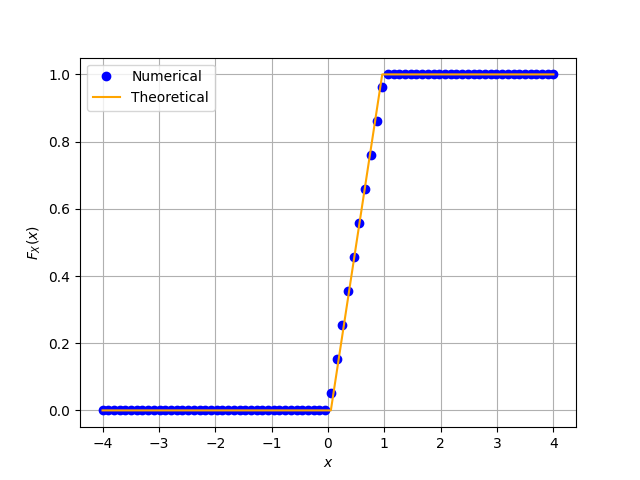
\includegraphics[width=\columnwidth]{1.2.png}
\caption{The CDF of $U$}
\label{fig:1.2}
\end{figure}
%
\item
Find a  theoretical expression for $F_{U}(x)$.\\
\solution\\ Given $U$ is a uniform Random Variable
\begin{align*}
p_{U}(x)=1 \text{ for } \\
F_U(x)=\int_{-\infty}^{\infty}p_{U}(x)dx\\
{\implies F_U(x)=
\begin{cases}
 0 &x\le0\\
 x &0< x< 1\\
 1 &x\ge 1
\end{cases}}
\end{align*}
\item
The mean of $U$ is defined as
%
\begin{equation}
E\sbrak{U} = \frac{1}{N}\sum_{i=1}^{N}U_i
\end{equation}
%
and its variance as
%
$
\text{var}\sbrak{U} = E\sbrak{U- E\sbrak{U}}^2 
$
Write a C program to  find the mean and variance of $U$. \\
\solution \\Download the following files and execute the  C program.\\
\begin{lstlisting}
wget https://github.com/kamujuaakash/Assignment1/blob/main/Exercise/Exercise-1/1.4/m.c
wget https://github.com/kamujuaakash/Assignment1/blob/main/Exercise/Exercise-1/1.4/coeffs.h
\end{lstlisting}
Download the above files and execute the following commands
\begin{lstlisting}
gcc m.c -lm
./a.out
\end{lstlisting}
\item Verify your result theoretically given that
\end{enumerate}
%
$$
E\sbrak{U^k} = \int_{-\infty}^{\infty}x^kdF_{U}(x)
$$
\solution \\
\begin{align*}
    E\sbrak{U}&=\int_{-\infty}^{\infty}xdF_U(x)\\
    E\sbrak{U}&=\int_{0}^{1}x\\
    \implies E\sbrak{U}=\frac{1}{2}\\
    E\sbrak{U^2}&=\int_{-\infty}^{\infty}x^{2}dF_U(x)\\
    E\sbrak{U^2}&=\int_{0}^{1}x^{2}dF_U(x)\\
    \implies E\sbrak{U^2}&=\frac{1}{3}\\
    \text{var}\sbrak{U} &= E\sbrak{U- E\sbrak{U}}^2\\ 
    \implies \text{var}\sbrak{U} &= E\sbrak{U^2}- E\sbrak{U}^2 
\end{align*}
$$ \boxed{\text{var}\sbrak{U}=\frac{1}{12}=0.0833}$$
\section{Central Limit Theorem}
%
\begin{enumerate}[label=\thesection.\arabic*
,ref=\thesection.\theenumi]
%
\item
Generate $10^6$ samples of the random variable
%
\begin{equation}
X = \sum_{i=1}^{12}U_i -6
\end{equation}
%
using a C program, where $U_i, i = 1,2,\dots, 12$ are  a set of independent uniform random variables between 0 and 1 and save in a file called gau.dat\\
\solution Download the following files and execute the  C program.
\begin{lstlisting}
wget https://github.com/kamujuaakash/Assignment1/blob/main/Exercise/Exercise-2/2.1/exrand.c
wget https://github.com/kamujuaakash/Assignment1/blob/main/Exercise/Exercise-2/2.1/coeffs.h
\end{lstlisting}
Download the above files and execute the following commands
\begin{lstlisting}
gcc exrand.c -lm
./a.out
\end{lstlisting}
\item
Load gau.dat in python and plot the empirical CDF of $X$ using the samples in gau.dat. What properties does a CDF have?\\
\solution \\
\begin{itemize}
\item $F_X (x)=P(X \leq x) $
\item $Q_X (x) = P(X > x)$
\item $Q_X (x) =\frac{1}{\sqrt{2\pi}} \int_{x} ^{\infty} e^{-\frac{u^2}{2}} du$
\item  $F_X (x) = 1 - Q_X (x)$ This can be used to calculate F (x).
\end{itemize}
The CDF of $X$ is plotted in Fig. \ref{fig:2.2}\\
using the code below
\begin{lstlisting}
wget https://github.com/kamujuaakash/Assignment1/blob/main/Exercise/Exercise-2/2.2/2.2.py
\end{lstlisting}
Download the above files and execute the following commands to produce Fig.\ref{fig:2.2}
\begin{lstlisting}
python3 2.2.py
\end{lstlisting}
\begin{figure}[!h]
\centering
\includegraphics[width=\columnwidth]{2.2.png}
\caption{The CDF of $X$}
\label{fig:2.2}
\end{figure}
Some of the properties of CDF 

     1) $$\lim_{x \to \infty}F_X(x) = 1$$\\
     2) $F_X(x)$ is non decreasing function.\\
     3) Symmetric about one point.

\item
Load gau.dat in python and plot the empirical PDF of $X$ using the samples in gau.dat. The PDF of $X$ is defined as
\begin{align}
p_{X}(x) = \frac{d}{dx}F_{X}(x)
\end{align}
What properties does the PDF have?
\\
\solution The PDF of $X$ is plotted in Fig. \ref{fig:2.3} using the code below
\begin{lstlisting}
wget https://github.com/kamujuaakash/Assignment1/blob/main/Exercise/Exercise-2/2.3/2.3.py
\end{lstlisting}
Download the above files and execute the following commands to produce Fig.\ref{fig:2.3}
\begin{lstlisting}
python3 2.3.py
\end{lstlisting}
\begin{figure}[!h]
\centering
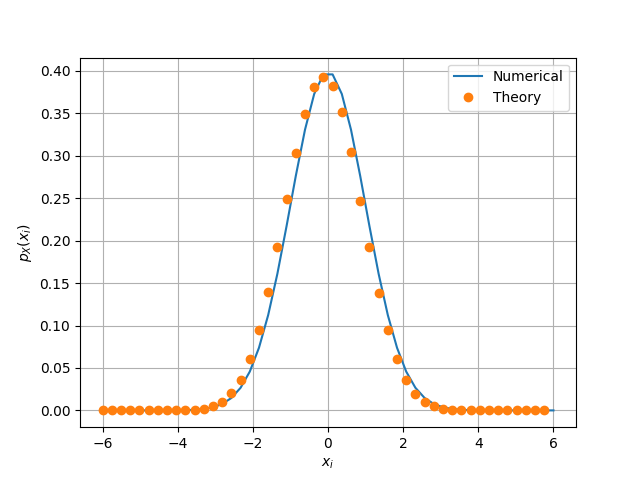
\includegraphics[width=\columnwidth]{2.3.png}
\caption{The PDF of $X$}
\label{fig:2.3}
\end{figure}
$$\text{Let }\mu \approx 0$$
Some of the properties of the PDF:
\begin{enumerate}
    \item Symmetric about $x=\mu$ in this case
    \item Decreasing function for $x>\mu$ and increasing for $x<\mu$ and attains maximum at $x=\mu$
    \item Area under the curve is unity.
\end{enumerate}
\item Find the mean and variance of $X$ by writing a C program.\\
\solution Download the following files and execute the  C program.
\begin{lstlisting}
wget https://github.com/kamujuaakash/Assignment1/blob/main/Exercise/Exercise-2/2.4/m.c
wget https://github.com/kamujuaakash/Assignment1/blob/main/Exercise/Exercise-2/2.4/coeffs.h
\end{lstlisting}
Download the above files and execute the following commands
\begin{lstlisting}
gcc m.c -lm
./a.out
\end{lstlisting}
\item Given that 
\begin{align}
p_{X}(x) = \frac{1}{\sqrt{2\pi}}\exp\brak{-\frac{x^2}{2}}, -\infty < x < \infty,
\end{align}
repeat the above exercise theoretically.
\end{enumerate}
\solution 
\begin{enumerate}
    \item CDF is given by 
    \begin{align}
        F_X(x)&=\int_{-\infty}^{\infty}p_X(x)dx\\
        \boxed{F_X(x)=1}
    \end{align}
    \item Mean is given by
    \begin{align*}
        E(x)=\int_{-\infty}^{\infty}xp_X(x)dx\\
        \int_{-\infty}^{\infty} \brak{x exp\brak{-\frac{x^2}{2}}dx}\\
        \text{Since the above function is odd}\\
        \implies \boxed{E(x)=0}
    \end{align*}
    \item Variance is given by
    \begin{align*}
        \text{var}\sbrak{U}&=E(U^2)-(E(U))^2\\
E\brak{x^2}&=\int_{-\infty}^{\infty}x^2p_X(x)dx \\
&=\int_{-\infty}^{\infty}\frac{1}{\sqrt{2\pi}}x^2exp\brak{-\frac{x^2}{2}}dx \\
&=\frac{1}{\sqrt{2\pi}}\brak{x\int_{-\infty}^{\infty} x exp\brak{-\frac{x^2}{2}}dx}
\\ &  -\frac{1}{\sqrt{2\pi}}\int_{-\infty}^{\infty}\brak{ \int \brak{x exp\brak{-\frac{x^2}{2}}dx}. dx}\\
\end{align*}
    
\begin{align*}
&=\left[-x\frac{1}{\sqrt{2\pi}} exp{\frac{-x^2}{2}}\right]_{-\infty}^{\infty}+\\ &\frac{1}{\sqrt{2\pi}}\int_{-\infty}^{\infty}exp\brak{-\frac{x^2}{2}}dx \\
&=\frac{\sqrt{2\pi}}{\sqrt{2\pi}}\\&=1
        \implies\boxed{\text{var}\sbrak{U}=1}
    \end{align*}
\end{enumerate}
\section{From Uniform to Other}
\begin{enumerate}[label=\thesection.\arabic*,ref=\thesection.\theenumi]
\item
Generate samples of 
%
\begin{equation}
V = -2\ln\brak{1-U}
\end{equation}
%
and plot its CDF.\\ 
\solution
Running the below code generates samples of V from file uni.dat(U).
\begin{lstlisting}
https://github.com/kamujuaakash/Assignment1/blob/main/Exercise/Exercise-3/3.1/3.1.py
\end{lstlisting}
Use the below command in the terminal to run the code:
\begin{lstlisting}
python3 3.1.py
\end{lstlisting}
Now these samples are used to plot  by running the below code,
 \begin{figure}[!h]
\includegraphics[width=0.5\textwidth]{3.2.png}
\caption{CDF for (3)}
\label{fig:V}
\end{figure}
\begin{lstlisting}
wge https://github.com/kamujuaakash/Assignment1/blob/main/Exercise/Exercise-3/3.1/cdf.py
\end{lstlisting}
Use the below command to run the code:
\begin{lstlisting}
python3 cdf.py
\end{lstlisting}
\item
Theorotical expression for $F_V (x)$
\begin{align*}
    F_V (x) &= P\{V \le x\} \\
            &= P\{-2\times \ln{(1-U)} \le x\} \\
            &= P\{U \le 1 - e^{(-\frac{x}{2})}\} \\ 
            &= F_U\{1- e^{(-\frac{x}{2})} \}\\
            &=
\begin{cases}
 1 - e^{(-\frac{x}{2})} & 0 \le x < \infty \\
 0  & x<0 \\
 \end{cases}
\end{align*} 
%Generate the Rayleigh distribution from Uniform. Verify your result through graphical plots.
\end{enumerate}
\section{Triangular Distribution}
\begin{enumerate}[label=\thesection.\arabic*
,ref=\thesection.\theenumi]
    \item Generate
    \begin{align}
        T=U_1+U_2
    \end{align}
    \solution Download the following files and execute the  C program.
\begin{lstlisting}
wget https://github.com/kamujuaakash/Assignment1/blob/main/Exercise/Exercise-4/4.1/4.1.c
wget https://github.com/kamujuaakash/Assignment1/blob/main/Exercise/Exercise-4/4.1/coeffs.h
\end{lstlisting}
Download the above files and execute the following commands
\begin{lstlisting}
gcc 4.1.c 
./a.out
\end{lstlisting}
\item Find the CDF of $T$.\\
\solution \\The CDF of $T$ is plotted in figure using the code below
\begin{lstlisting}
wget https://github.com/kamujuaakash/Assignment1/blob/main/Exercise/Exercise-4/4.2/4.2.py
\end{lstlisting}
\begin{figure}[!h]
\centering
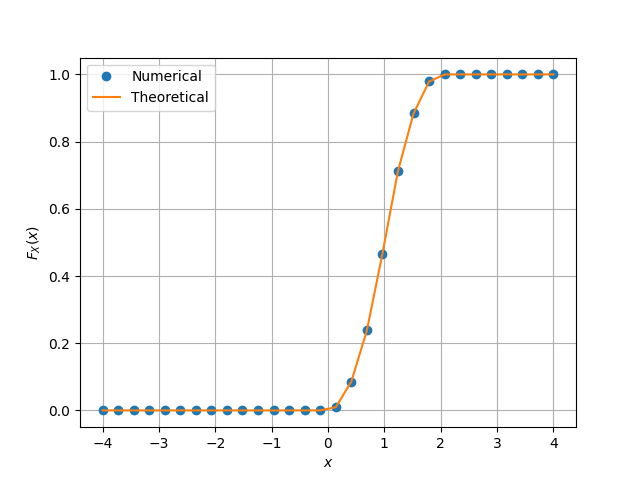
\includegraphics[width=\columnwidth]{4.2.png}
\caption{The CDF of $T$}
\label{fig:4.2}
\end{figure}
Download the above files and execute the following commands to produce Fig.\ref{fig:4.2}
\begin{lstlisting}
python3 4.2.py
\end{lstlisting}

\item Find the PDF of $T$.\\
\solution\\ 
\begin{figure}[!h]
\centering
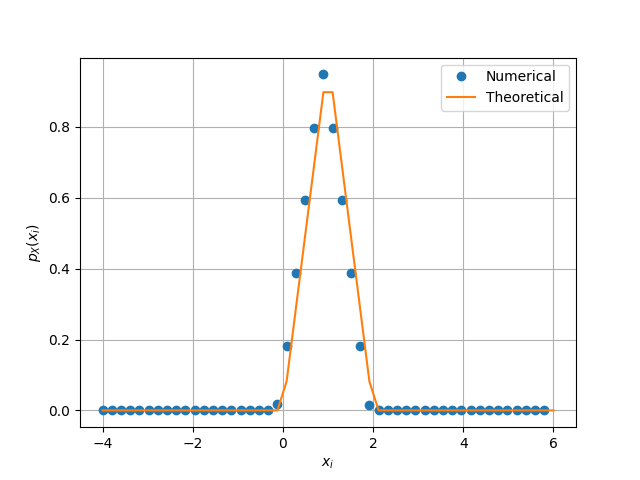
\includegraphics[width=\columnwidth]{4.3.png}
\caption{The PDF of $T$}
\label{fig:4.3}
\end{figure}
The PDF of $T$ is plotted in Fig. \ref{fig:4.2} using the code below
\begin{lstlisting}
wget https://github.com/kamujuaakash/Assignment1/blob/main/Exercise/Exercise-4/4.3/4.3.py
\end{lstlisting}
Download the above files and execute the following commands to produce Fig.\ref{fig:4.2}
\begin{lstlisting}
python3 4.3.py
\end{lstlisting}

\item Find the Theoretical Expression for the PDF and CDF of $T$\\
\solution
\begin{align}
    T&=U_1+U_2\\
    \implies p_T(t)&=\int_{-\infty}^{t}p_{U1}(x)p_{U2}(y)dx\\
    \text{As,}p_{U1}(x)&=p_{U1}(y)=p_{U}(u)\\
    \implies p_T(t)&=\int_{-\infty}^{t}p_{U}(u)p_{U}(t-u)du
    \end{align}
    \begin{enumerate}
        \item Theoretical PDF 
        \begin{enumerate}
            \item $t\le 1$
            \begin{align}
                p_T(t)&=\int_{0}^{t}p_{U}(t-u)du\\
                \implies p_T(t)&=\int_{0}^{t} du=t
            \end{align}
            \item $t> 1$
             \begin{align}
                p_T(t)&=\int_{0}^{1}p_{U}(t-u)du\\
                \implies p_T(t)&=\int_{t-1}^{1} du=2-t
            \end{align}
        \end{enumerate}
        $\implies\boxed{ P_T(t) =
        \begin{cases}
         t     &0 \le t \le 1 \\
         2-t   &1 < t \le 2\\
         0     &t<0 \text{ or }t>2
        \end{cases}
        }$\\
        \item Theoretical CDF 
        \begin{align}
            F_T(t)=\int_{-\infty}^{t}p_T(u)du
        \end{align}
        $\implies\boxed{
            F_{T}(t)=
            \begin{cases}
             0   &t<0\\
             \dfrac{t^2}{2} &0\le t \le 1\\
             2t-1-\dfrac{t^2}{2} &1<t \le 2\\
             1 &t>2
            \end{cases}
            }$\\
    \end{enumerate}
\item Verify your results through a plot \\
\solution The Results are verified in the plots in Fig.\ref{fig:4.2}and Fig.\ref{fig:4.3}\section{Maximum Likelihood}
\begin{enumerate}[label=\thesection.\arabic*
,ref=\thesection.\theenumi]
\item Generate equiprobable $X \in \cbrak{1,-1}$.\\	
  \solution The generating X or bernoulie random variable $ \brak{X}$ is done by using uni.dat file. Download the below files
    \begin{lstlisting}
         wget https://github.com/kamujuaakash/Assignment1/blob/main/Exercise/Exercise-5/coeffs.h
	 wget https://github.com/kamujuaakash/Assignment1/blob/main/Exercise/Exercise-5/5.1.c
    \end{lstlisting}
  Run the following command
    \begin{lstlisting}
	  gcc 5.5.c -lm
	  ./a.out 
    \end{lstlisting} 
\item Generate
$
Y = AX+N,
$
	where $A = 5$ dB,  and $N \sim {0}{1}$.\\
  \solution To generate distribution of Y random variable we will need previously generated bernoulie distribution and gaussian distribution.Download the below files
    \begin{lstlisting}
     wget  https://github.com/kamujuaakash/Assignment1/blob/main/Exercise/Exercise-5/coeffs.h
     wget https://github.com/kamujuaakash/Assignment1/blob/main/Exercise/Exercise-5/5.2.c
    \end{lstlisting}
   Then run the following command,
    \begin{lstlisting}
     gcc 5.2.c -lm
     ./a.out
    \end{lstlisting}
\item Plot $Y$ using a scatter plot.\\
 \solution Download the below files
    \begin{lstlisting}
      wget https://github.com/kamujuaakash/Assignment1/blob/main/Exercise/Exercise-5/5.3.py
    \end{lstlisting}
   Then run the following command,
    \begin{lstlisting}
      python3 5.3.py
    \end{lstlisting}	
   	\begin{figure}
   		\centering
   		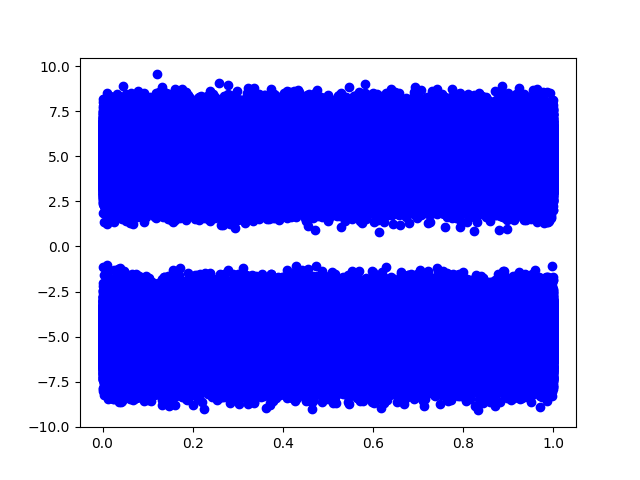
\includegraphics[width=\columnwidth]{5.3.png}
   		\caption{The scatter plot of $Y$}
   		\label{fig:Y_scatterplot}
   	\end{figure}
\item Guess how to estimate $X$ from $Y$.\\
	\solution When $ Y > 0 $, we can more probably say that $X = 1$ as $X$ can take values from $\sbrak{-1,1}$.As $A$ increases the signal contribution will increase compared to noise.The scatter plot will not be intermixed as $A$ increases. So in this case, the scatter plot of $Y$ is seperated with decision boundary as $0$. So we can more probably say that,
	  \begin{align}
		  X &= \begin{cases}
			  1 &, Y>0\\
			 -1 &, Y<0 
		       \end{cases}
          \end{align}		       
\item
\label{ml-ch4_sim}
Find
\begin{equation}
	P_{e|0} = \pr{\hat{X} = -1|X=1}
\end{equation}
and
\begin{equation}
	P_{e|1} = \pr{\hat{X} = 1|X=-1}
\end{equation}
%
\solution The $\hat{X}$ is defined as,
  \begin{align}
      \hat{X} &= \begin{cases}
	             1  &, Y > 0\\
		     0  &, Y\leq 0
		 \end{cases}
  \end{align}
 The error probability, when the actual signal is $X=1$ but transmitted as $\hat{X} = -1$ is,
  \begin{align}
	  P_{e|0} &= \pr{\hat{X} = -1|X=1}\\
	          &= \pr{ Y \leq 0| X= 1}\\
		  &= \pr{AX + N \leq 0 | X=1}\\
		  &= \pr{ A + N \leq 0}\\
		  &= \pr{N \leq -A}\\
		  &= F_{N}\brak{-A}\\
		  &= 1 - Q\brak{-A}\\
		  &= 2.866515718791946e-07\label{eq:5-5-1}
  \end{align}
 And for the case when actual signal is $X=-1$ but transmitted as $\hat{X} = 1$ the error probability will be,
  \begin{align}
	  P_{e|1} &= \pr{\hat{X} = 1|X=-1}\\
                  &= \pr{ Y > 0| X=-1}\\
                  &= \pr{AX + N > 0 | X=1}\\
                  &= \pr{ N-A > 0}\\
                  &= \pr{N > A}\\
		  &= 1 - F_{N}\brak{A}\\
		  &= Q\brak{A}\\
		  &= 2.866515719235352e-07\label{eq:5-5-2}
  \end{align}
The above calculations are coded in below python file,
  \begin{lstlisting}
    wget  https://github.com/kamujuaakash/Assignment1/blob/main/Exercise/Exercise-5/5.5.py
  \end{lstlisting}
  Run the following command
  \begin{lstlisting}
   python3 5.5.py
  \end{lstlisting}
\item Find $P_e$ assuming that $X$ has equiprobable symbols.\\
 \solution Given that $X$ has equiprobable symbols so,
   \begin{align}
	   \pr{X = 1} &= \frac{1}{2}\\
	   \pr{X=-1}  &= \frac{1}{2}
   \end{align}
   	From total probability theorem,
   \begin{align}
	   P_{e} &= \pr{e|1}\pr{X = -1} + \pr{e|0}\pr{X=1}\\
		       &= \frac{1}{2}\brak{\pr{e|1} + \pr{e|0}}
   \end{align}
From $\eqref{eq:5-5-1}$,$\eqref{eq:5-5-2}$
   \begin{align}
	   \pr{e} &= 2.866515719013649e-07 
   \end{align}
\item
Verify by plotting  the theoretical $P_e$ with respect to $A$ from 0 to 10 dB.\\
 \solution
   We know,
     \begin{align}
	     P_e  &= P_{e|1}\pr{X = -1} + P_{e|0}\pr{X=1} \\
		  &= \frac{1}{2}\brak{ 1 - Q\brak{-A}} + \frac{1}{2}\brak{Q\brak{A}}
     \end{align}
    The above mentioned is the theoritical expression of $P_e$ w.r.t to $A$, it is plotted in rectangular axes and semi-log y axes using the below python codes,
    \begin{lstlisting}
     wget https://github.com/kamujuaakash/Assignment1/blob/main/Exercise/Exercise-5/5.7.py
    \end{lstlisting}
Then the following commands
    \begin{lstlisting}
      python3 5.7.py
    \end{lstlisting}
\begin{figure}
  \centering
  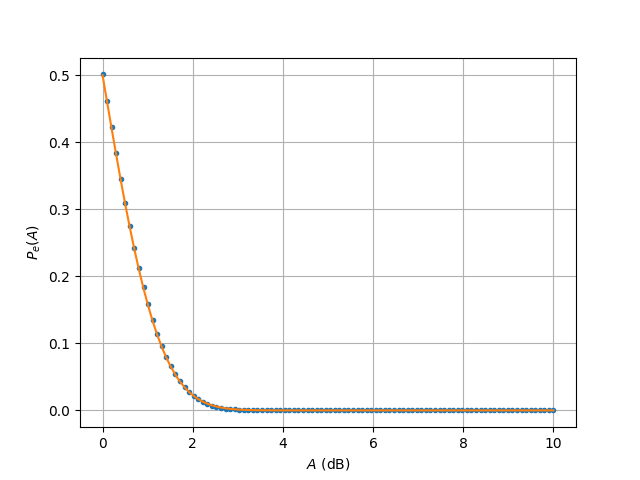
\includegraphics[width=\columnwidth]{5.7.png}
  \caption{$P_e$ vs $A$}
  \label{fig:P_e_A}
 \end{figure}
%
\item Now, consider a threshold $\delta$  while estimating $X$ from $Y$. Find the value of $\delta$ that maximizes the theoretical $P_e$.\\
 \solution
     \begin{align}
	     P_{e|0} &= \pr{\hat{X} = -1|X = 1}\\
		     &= \pr{Y \leq \delta| X =1}\\
                     &= \pr{AX + N \leq \delta | X =1}\\
		     &= \pr{A + N \leq \delta}\\
		     &= \pr{ N \leq \delta -A}\\
		     &= F_{N}\brak{\delta-A}\\
		     &= 1- Q\brak{\delta -A}
     \end{align}
     And,
     \begin{align}
	    P_{e|1} &= \pr{\hat{X} = 1|X = -1}\\
	            &= \pr{Y > \delta| X =-1}\\
                    &= \pr{AX + N > \delta | X =-1}\\
                    &= \pr{N - A > \delta}\\ 
                    &= \pr{ N > \delta + A}\\
                    &= Q\brak{\delta + A}
     \end{align}     
  So we can write,
     \begin{align}
	     P_e &= P_{e|1}\pr{X = -1} + P_{e|0}\pr{X=1}\label{eq:5-8}\\
	         &=\frac{1}{2}\brak{ 1 -Q\brak{\delta -A}  + Q\brak{\delta + A}}
     \end{align}
  Now to maximize the $P_e$, we will differentiate the expression w.r.t $\delta$ and equate it to $0$.
     \begin{align}
	     \frac{dP_e}{d\delta} = \frac{d}{d\delta}\brak{1 -Q\brak{\delta -A}  + Q\brak{\delta + A}} = 0\\
	              \implies      \frac{d}{d\delta}\brak{F_{N}\brak{\delta - A} + 1 - F_{N}\brak{\delta +A}} &= 0\\
	              \implies       p_{N}\brak{\delta -A} - p_{N}\brak{\delta + A} &= 0 \\
				             \exp\brak{-\frac{\brak{\delta-A}^2}{2}} \nonumber  - \exp\brak{-\frac{\brak{\delta+A}^2}{2}}  &= 0
     \end{align}
     Since $e^x$ is one - one function, we can write,
     \begin{align}
	    - \frac{\brak{\delta - A}^2}{2} &= -\frac{\brak{\delta + A}^2}{2}\\
		  \brak{\delta - A}^2 &= \brak{\delta + A}^2\\
		  \delta &= 0 
     \end{align}
    Now we will find whether $P_e$ attains maxima or minima at $\delta = 0$
     \begin{align}
	     \frac{d^2P_e}{d\delta^{2}}|_{\delta = 0} &= 2A\exp\brak{\frac{-A^{2}}{2}} > 0
     \end{align}
\item Repeat the above exercise when
	\begin{align}
		p_{X}(0) = p
	\end{align}
 \solution Given that,
         \begin{align}
		 p_{X}\brak{0} = p
         \end{align}
	 So,
	 \begin{align}
           \pr{X = 1} = p_{X}\brak{0} = p\\
           \pr{X = -1} &= 1 - p
         \end{align}		 
   From $\eqref{eq:5-8}$ we can write
         \begin{align}
             P_e &= P_{e|1}\pr{X = -1} + P_{e|0}\pr{X=1} \\
		 &= \brak{1-p}Q\brak{\delta + A} + p\brak{1 - Q\brak{\delta - A}}\\
		 &= \brak{1-p}Q\brak{\delta + A} + pQ\brak{A - \delta}
         \end{align}
   Now to maximize the $P_e$, we will differentiate the expression w.r.t $\delta$ and equate it to $0$.
         \begin{align}
          &\frac{d}{d\delta}P_e=p\frac{d}{d\delta} Q\brak{A -\delta}\nonumber \\
          &+\brak{1-p}\frac{d}{d\delta} Q_N\brak{A+\delta}=0\\
          &p\frac{d}{d\delta} F_N\brak{-A+\delta}\nonumber \\
          &+\brak{1-p}\frac{d}{d\delta}\brak{1-F_N\brak{A+\delta}}=0\\
          &\implies p\times p_N\brak{-A+\delta}\\
          &-\brak{1-p}p_N\brak{A+\delta}=0
         \end{align}     
  From the PDF of gaussian, we will get
         \begin{align}
		 \delta &= \frac{\ln\brak{\frac{1}{p} - 1}}{2A}
         \end{align}
\item Repeat the above exercise using the MAP criterion.\\
  \solution From the Bayes theorem, we can write
       \begin{align}
	          &\pr{X=1|Y=y}  \\
	          &= \frac{\pr{X=1,Y=y}}{\pr{Y=y}}\\
		      &= \frac{p\pr{N = y -A}}{pP_{Y|X}\brak{y|1} +\brak{1-p}P_{Y|X}\brak{y|-1}}\\
		      &= \frac{p p_{N}\brak{y-A}}{pp_{N}\brak{y-A} + \brak{1-p}p_{N}\brak{y+A}}\\
		      &= \frac{p}{p + \brak{1-p}\exp\brak{-2yA}}
       \end{align}
       And similarly for,
       \begin{align}
	          &\pr{X=-1|Y=y} \\
	          &= \frac{\pr{X=-1,Y=y}}{\pr{Y=y}}\\
		      &= \frac{\brak{1-p}\pr{N = y +A}}{pP_{Y|X}\brak{y|1} +\brak{1-p}P_{Y|X}\brak{y|-1}}\\
		      &= \frac{\brak{1-p}p_{N}\brak{y+A}}{pp_{N}\brak{y-A} + \brak{1-p}p_{N}\brak{y+A}}\\
              &= \frac{1-p}{1-p+ p\exp{2yA}}
       \end{align}
       Now for a particular y, to make $X = 1$ more likely than $X= -1$,
        \begin{align}
	   &\pr{X=1|Y=y} > \pr{X=-1|Y=y}\\
	   &\frac{p}{p + \brak{1-p}\exp\brak{-2yA}} >\frac{1-p}{1-p+ p\exp\brak{2yA}}\\
	   &p^2e^{2yA} > \brak{1-p}^{2}e^{-2yA}\\
       &e^{2yA} >\frac{1-p}{p}\\
	   &y > \frac{\ln{\brak{\frac{1-p}{p}}}}{2A}
	\end{align}
	And similarly for a particular y, to make $X=-1$ more likely than $X=1$, we need
	 \begin{align}
		 y < \frac{\ln{\brak{\frac{1-p}{p}}}}{2A}
         \end{align}
	 So to minimise the $P_e$ we need a threshold of
	  \begin{align}
		  \delta &= \frac{\ln{\brak{\frac{1-p}{p}}}}{2A}
          \end{align}		   
  \end{enumerate}
\section{Gaussian to Other}
\begin{enumerate}[label=\thesection.\arabic*
,ref=\thesection.\theenumi]
\item
%Let $X_1 \sim  \gauss{0}{1}$ and $X_2 \sim  \gauss{0}{1}$. Plot the CDF and PDF of
%
\begin{equation}
V = X_1^2 + X_2^2
\end{equation}
 \solution Download the below files to generate the random variable $V$,
	 \begin{lstlisting}
          
         \end{lstlisting}
	Then run the following command,
	 \begin{lstlisting}
	  
	 \end{lstlisting}
	 For CDF download the below python file,
	 \begin{lstlisting}
	 
	 \end{lstlisting}
	 Then run the following command,
	\begin{lstlisting}
          
        \end{lstlisting}
       For PDF download the below pyhon file,
	\begin{lstlisting}

        \end{lstlisting}
       Then run the follwing terminal in terminal,
	\begin{lstlisting}
	 
	\end{lstlisting}
    %\begin{figure}
     %\centering
     %\includegraphics[width=\columnwidth]{Q6/chi_square_cdf.png}
     %\caption{The CDF of $V$}
     %\label{fig:V_Cdf}
    %\end{figure}
     %\begin{figure}
     %\centering
     %\includegraphics[width=\columnwidth]{Q6/chi_squared_pdf.png}
     %\caption{The PDF of $V$}
     %\label{fig:V_PDF}
    %\end{figure}
%
%
%
\item
If
%
\begin{equation}
F_{V}(x) =
\begin{cases}
1 - e^{-\alpha x} & x \geq 0 \\
0 & x < 0,
\end{cases}
\end{equation}
%
find $\alpha$.\\
%
\item
\label{ch3_raleigh_sim}
Plot the CDF and PDf of
%
\begin{equation}
A = \sqrt{V}
\end{equation}
%
\end{enumerate}
\section{Conditional Probability}
\begin{enumerate}[label=\thesection.\arabic*
,ref=\thesection.\theenumi]
\item
\label{ch4_sim}
Plot
\begin{equation}
P_e = \pr{\hat{X} = -1|X=1}
\end{equation}
%
for
\begin{equation}
Y = AX+N,
\end{equation}
%where $A$ is Raleigh with $E\sbrak{A^2} = \gamma, N \sim \gauss{0}{1}, X \in \brak{-1,1}$ for $0 \le \gamma \le 10$ dB.
%
\item
Assuming that $N$ is a constant, find an expression for $P_e$.  Call this $P_e(N)$
%
\item
%
\label{ch4_anal}
For a function $g$,
\begin{equation}
E\sbrak{g(X)} = \int_{-\infty}^{\infty}g(x)p_{X}(x)\, dx
\end{equation}
%
Find $P_e = E\sbrak{P_e(N)}$.
%
\item
Plot $P_e$ in problems \ref{ch4_sim} and \ref{ch4_anal} on the same graph w.r.t $\gamma$.  Comment.
		\end{enumerate}
\section{Two Dimensions}
Let
\begin{equation}
\mbf{y} = A\mbf{x} + \mbf{n},
\end{equation}
where
\begin{align}
x &\in \brak{\mbf{s}_0,\mbf{s}_1},
\mbf{s}_0 =
\begin{pmatrix}
1
\\
0
\end{pmatrix},
\mbf{s}_1 =
\begin{pmatrix}
0
\\
1
\end{pmatrix}
\\
\mbf{n} &=
\begin{pmatrix}
n_1
\\
n_2
\end{pmatrix},
n_1,n_2 \sim {0}{1}.
\end{align}
%
\begin{enumerate}[label=\thesection.\arabic*
,ref=\thesection.\theenumi]
%%
\item
\label{ch5_fsk}
Plot
%
\begin{equation}
\mbf{y}|\mbf{s}_0 \text{ and } \mbf{y}|\mbf{s}_1
\end{equation}
%
on the same graph using a scatter plot.
%
\item
For the above problem, find a decision rule for detecting the symbols $\mbf{s}_0 $ and $\mbf{s}_1$.
%
\item
Plot
\begin{equation}
P_e = \pr{\hat{\mbf{x}} = \mbf{s}_1|\mbf{x} = \mbf{s}_0}
\end{equation}
with respect to the SNR from 0 to 10 dB.
%
\item
Obtain an expression for $P_e$. Verify this by comparing the theory and simulation plots on the same graph.
%
		\end{enumerate}

\end{enumerate}
\end{document}
